\documentclass[../Main.tex]{subfiles}

\begin{document}

\section{Design und Umsetzung des Kampfabschnitts} \label{sec:Umsetzung}

In diesem Kapitel werden zunächst Designvorschläge für die beiden inhaltlichen Komponenten der Erkenntnisfrage (Abschnitt~\ref{sec:Erkenntnisfrage}) aufgestellt: Gegnerverhalten einerseits, Gegnerplatzierung und Leveldesign andererseits. Sie zielen auf die drei dort genannten spielerischen Qualitäten ab, nämlich einen nachvollziehbaren Spielfluss, eine angemessene Schwierigkeit und ein befriedigendes Spielgefühl. Dazu werden die Erkenntnisse aus der Referenzspielanalyse (Kapitel~\ref{sec:Referenzspielanalyse}) besonders für das Gegnerverhalten gewonnen und der Leveldesign-Recherche (Kapitel~\ref{sec:Leveldesign}) vor allem für die Gegnerplatzierung zu spezifischen Designvorschlägen für unseren Kampfabschnitt verdichtet. Nicht alle Punkte aus der Recherche konnten in den Designvorschlägen berücksichtigt werden, da dies im vorgegebenen Zeitraum nicht möglich war. Deshalb haben wir jene Punkte ausgewählt, die wir als besonders wichtig für unsere Erkenntnisfrage oder als im Prototyp überprüfbar eingeschätzt haben. Wie wir diese Designvorschläge spezifisch umgesetzt haben oder welche software wir dafür benutzt haben, ist alles in kapitel 2.5 notiert. Für jeden Vorschlag wird beschrieben, wie er im Prototyp umgesetzt wurde und wo sich die Umsetzung überprüfen lässt. Die Überprüfung mittels Playtests folgt in Kapitel~\ref{sec:Evaluation} der Playtests ist auch der Massstab an dem wir die oben genannten spielerischen Qualitäten überprüfen.

\begin{itemize}[leftmargin=1.5cm]
    \item \textcolor{red}{\textbf{Vorgehen (1--2 Sätze):} Erinnerung, wie umgesetzt wurde (Greybox in TrenchBroom, Godot, iterativ), mit Verweis auf Abschnitt~\ref{sec:VorgehenUmsetzung}.}
    \item \textcolor{red}{\textbf{Verweise auf die Erkenntnisse:} \enquote{Dazu werden die Erkenntnisse \ldots\ verdichtet} -- hier direkt auf die beiden neuen Abschnitte verweisen: Erkenntnisse aus den Analysen (Abschnitt~\ref{sec:Vergleich}, 3.3.3) und aus der Leveldesign-Recherche (Abschnitt~\ref{sec:ZwischenfazitLD}).}
    \item \textcolor{red}{\textbf{Arbeitsteilung sichtbar machen (1 Satz):} Die Vorschläge zum Gegnerverhalten (V1--V4) stammen vor allem aus Kapitel~\ref{sec:Referenzspielanalyse}, jene zur Gegnerplatzierung und zum Kampfraum (V5--V8) vor allem aus Kapitel~\ref{sec:Leveldesign}. So steht es auch in 4.7.}
    \item \textcolor{red}{\enquote{da dies im vorgegebenen Zeitraum nicht möglich war}: Zeitmangel als Grund ist ehrlich, gehört aber eher in die Limitationen (Abschnitt~\ref{sec:Limitationen}). Hier reicht das Auswahlkriterium (wichtig für die Erkenntnisfrage, im Prototyp prüfbar).}
\end{itemize}

\subsection{Von der Recherche zu den Designvorschlägen} \label{sec:Designvorschlaege}

Hier in diesem Abschnitt nennen wir unsere ausgewählten designziele und listen sie übersichtlich auf. hier nennen wir nur ihre namen und zeigen auf aus welchem teil unserer langen recherche wir sie her haben. in den folgenden kapiteln wird jeder dieser Designvorschläge genau aufgeschlüsselt. Jeder Designvorschlag folgt demselben Schema: der Vorschlag selbst, sein Nutzen, also welcher Aspekt der Erkenntnisfrage damit bedient wird, und die Herleitung aus Recherche und Spielanalysen. Die Vorschläge sind mit V1 bis V8 nummeriert; die tabelle unten, Tabelle~\ref{tab:Designvorschlaege} gibt einen Überblick über die Vorschläge und ihre Herleitung.

\begin{table}[H]
    \centering
    \small
    \renewcommand{\arraystretch}{1.3}
    \begin{tabular}{|>{\raggedright\arraybackslash}p{0.6cm}|>{\raggedright\arraybackslash}p{4.8cm}|>{\raggedright\arraybackslash}p{8.4cm}|}
        \hline
        \textbf{Nr.} & \textbf{Designvorschlag} & \textbf{Herleitung} \\
        \hline
        \multicolumn{3}{|l|}{\textit{Gegnerverhalten (Abschnitt~\ref{sec:UmsetzungGegner})}} \\
        \hline
        V1 & Überlegenheit als Grundzustand & Kontrast \game{NieR: Automata} / \game{Ninja Gaiden} (Abschnitte~\ref{sec:ReferenzspielanalyseNier} und~\ref{sec:ReferenzspielanalyseNinja}); emotionsgeleitetes Design (Abschnitt~\ref{sec:Pacing}) \\
        \hline
        V2 & Begrenzung gleichzeitiger Angreifer & Beide Referenzspiele (Abschnitt~\ref{sec:Vergleich}); Pacing (Abschnitt~\ref{sec:Pacing}) \\
        \hline
        V3 & Taktisches Dilemma durch zwei Gegnerrollen & Frage D2 beider Analysen; Gegnerrollen im Encounter-Design (Abschnitt~\ref{sec:Encounter}) \\
        \hline
        V4 & Klar telegrafierte Angriffe & \game{NieR: Automata}, Frage M2; Lesbarkeit (Abschnitt~\ref{sec:Encounter}) \\
        \hline
        \multicolumn{3}{|l|}{\textit{Gegnerplatzierung und Kampfraum (Abschnitt~\ref{sec:UmsetzungLevel})}} \\
        \hline
        V5 & Lesbare Platzierung, dynamisches Verhalten & \game{NieR: Automata}, Frage A3; \game{Ninja Gaiden}, Frage D3 (Abschnitt~\ref{sec:Vergleich}); Lesbarkeit (Abschnitt~\ref{sec:Encounter}) \\
        \hline
        V6 & Der Raum als Druckmittel & \game{Ninja Gaiden}, Frage M3; räumliche Typologien (Abschnitt~\ref{sec:Raumtypologien}) \\
        \hline
        V7 & Wellenstruktur mit Erholungsphasen & \game{Ninja Gaiden}, Frage D1; \game{NieR: Automata}, Frage A4; Rollercoaster-Pacing (Abschnitt~\ref{sec:Pacing}) \\
        \hline
        V8 & Gestaffelte Einführung neuer Gegner & Scaffolding (Abschnitt~\ref{sec:Scaffolding}); \game{NieR: Automata}, Frage D1 \\
        \hline
    \end{tabular}
    \caption{Übersicht der Designvorschläge und ihrer Herleitung}
    \label{tab:Designvorschlaege}
\end{table}

\begin{itemize}[leftmargin=1.5cm]
    \item \textcolor{red}{\textbf{Tabelle, Spalte Herleitung -- drei schwache Verweise:} V2 \enquote{Pacing (Abschnitt~\ref{sec:Pacing})} -- die Begrenzung der Angreifer kommt nicht aus dem Pacing, sondern nur aus Kapitel~\ref{sec:Referenzspielanalyse}. V3 \enquote{Gegnerrollen im Encounter-Design} -- das steht im roten Absatz zu \game{Ninja Gaiden} in 4.2, keine Leveldesign-Literatur; stattdessen Frage~D2 beider Analysen bzw.\ \game{NieR} D2 (Small Stubbies versperren den Weg). V4 \enquote{Lesbarkeit} -- in 4.2 geht es um die Lesbarkeit des Raums, nicht der Angriffe; nur \game{NieR} M2 angeben.}
    \item \textcolor{red}{\textbf{V5 in der Tabelle:} \enquote{Gegner als raumbildende Elemente} heisst in 4.2 und 4.7 \textit{Shrinking Fortress} -- denselben Begriff verwenden.}
    \item \textcolor{red}{\textbf{Begriff \enquote{Gegnerrollen} bei V3:} In der Analyse von \game{Ninja Gaiden} (Frage~M2) unterscheidet ihr ausdrücklich zwischen Gegner\emph{typ} (Nah-/Fernkämpfer) und \emph{Rolle} (Nahkämpfer, Flankierer, Fernkämpfer als situatives Verhalten). V3 meint die Typen. Umbenennen, z.\,B.\ \enquote{Taktisches Dilemma durch Nah- und Fernkämpfer} (auch in der Überschrift von V3 und in Kapitel~\ref{sec:Evaluation}).}
\end{itemize}

\subsection{Der Prototyp im Überblick} \label{sec:Prototyp}

\begin{itemize}[leftmargin=1.5cm]
    \item \textcolor{red}{1--2 Sätze: Was ist der Prototyp (3D, Third-Person, Godot, ein zusammenhängender Kampfabschnitt)? Kann fast wörtlich aus Abschnitt~\ref{sec:Aufbau} übernommen werden.}
\end{itemize}

\subsubsection{Spieler und Gegnertypen} \label{sec:Gegnertypen}

\begin{itemize}[leftmargin=1.5cm]
    \item \textcolor{red}{Zuerst kurz den Spieler vorstellen: Moveset (rennen, springen, Dash, Ledge Grab, Light-, Heavy- und Air-Combo, heilen). Details zu den Werten folgen unten.}
\end{itemize}

In unserem Prototyp gibt es zwei Gegnerklassen, Nah- und Fernkämpfer, von denen es jeweils mehrere Varianten gibt: zwei Nahkämpfer und drei Fernkämpfer. Insgesamt gibt es damit fünf verschiedene Gegnertypen (Abbildung~\ref{fig:Gegnertypen}). Farblich sind die Nahkämpfer in Rottönen und die Fernkämpfer in Gelb- bis Orangetönen gehalten.

\begin{figure}[H]
    \centering
    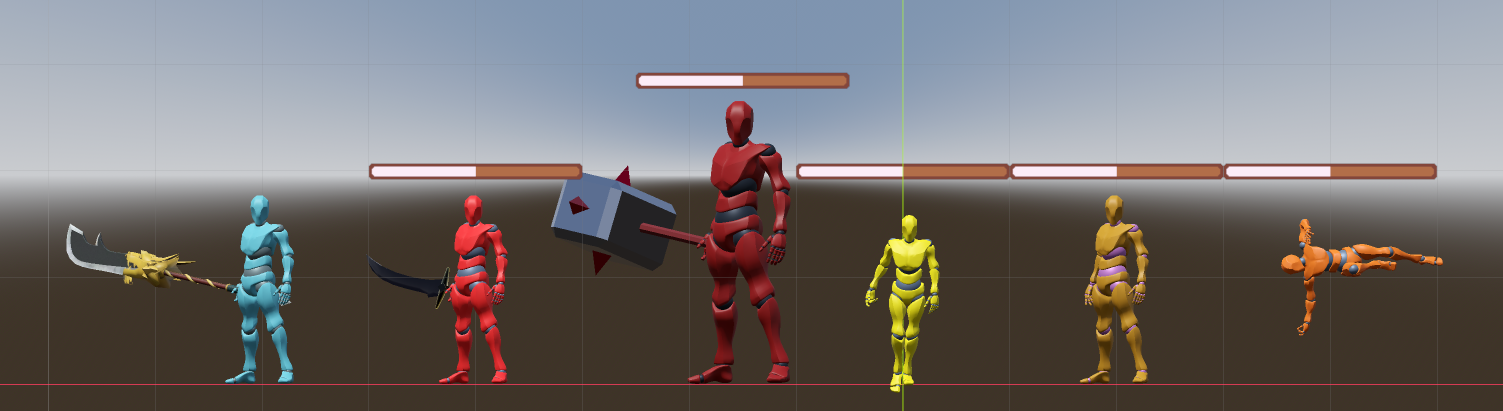
\includegraphics[width =\linewidth]{Assets/All Entities.png}
    \caption[Die fünf Gegnertypen des Prototyps. Eigene Abbildung.]{Die fünf Gegnertypen des Prototyps und der Spieler, von links nach rechts: Spieler (Blau), Soldier (Rot), Heavy Soldier (Dunkelrot), Archer (Gelb), Heavy Archer (Hellbraun), Chain Archer (Orange). Eigene Abbildung.}
    \label{fig:Gegnertypen}
\end{figure}

Der Soldier ist der grundlegende Nahkämpfer, der auf den Spieler zurennt und zuschlägt. Der Heavy Soldier ist grösser, stärker und langsamer als der Soldier und hat mehr Lebenspunkte, zeigt aber dasselbe Verhalten.

Die Fernkämpfer bewegen sich alle nicht. Der Archer schiesst ein Projektil auf den Spieler. Der Heavy Archer macht dasselbe, sein Projektil ist jedoch langsamer, kann dafür die Richtung ändern und verfolgt den Spieler. Der Chain Archer schiesst gleich drei Pfeile auf den Spieler, die mehr als doppelt so schnell sind wie jene des Archers.

Die Reichweite der Archers, also die Distanz, aus der sie auf den Spieler schiessen können, ist bei allen drei Typen gleich. Lebenspunkte und Schaden unterscheiden sich dagegen je nach Gegnertyp; Tabelle~\ref{tab:Gegnertypen} fasst die Eigenschaften zusammen.

\begin{table}[H]
    \centering
    \small
    \renewcommand{\arraystretch}{1.3}
    \begin{tabular}{|>{\raggedright\arraybackslash}p{2.3cm}|>{\raggedright\arraybackslash}p{2.9cm}|>{\raggedright\arraybackslash}p{3.0cm}|>{\raggedright\arraybackslash}p{0.8cm}|>{\raggedright\arraybackslash}p{1.4cm}|>{\raggedright\arraybackslash}p{1.9cm}|}
        \hline
        \textbf{Gegnertyp} & \textbf{Bewegung} & \textbf{Angriff} & \textbf{LP} & \textbf{Schaden} & \textbf{Unter\-brechbar} \\
        \hline
        \multicolumn{6}{|l|}{\textit{Nahkämpfer (Rottöne)}} \\
        \hline
        Soldier & rennt auf den Spieler zu & Nahkampfschlag & 130 & 15 & ja \\
        \hline
        Heavy Soldier & wie Soldier, aber langsamer; grösser & wie Soldier & 200 & 30 & nein \\
        \hline
        \multicolumn{6}{|l|}{\textit{Fernkämpfer (Gelb- bis Orangetöne)}} \\
        \hline
        Archer & stationär & ein Projektil & 60 & 10 & ja \\
        \hline
        Heavy Archer & stationär & ein langsameres, zielsuchendes Projektil & 40 & 20 & ja \\
        \hline
        Chain Archer & stationär & drei Pfeile, mehr als doppelt so schnell wie beim Archer & 70 & $3 \times 10$ & ja \\
        \hline
    \end{tabular}
    \caption{Eigenschaften der fünf Gegnertypen (LP = Lebenspunkte)}
    \label{tab:Gegnertypen}
\end{table}

\paragraph{Abstimmung von Schaden und Lebenspunkten}
Der Spieler selbst hat 200 Lebenspunkte. Er heilt jedes Mal 50 Lebenspunkte auf einmal; mit einer vollen Manaleiste kann er genau 200 Lebenspunkte heilen, also seine Lebenspunkte einmal vollständig wiederherstellen. Seine Angriffe verursachen je nach Combo unterschiedlich viel Schaden (Tabelle~\ref{tab:Combos}).

\begin{table}[H]
    \centering
    \small
    \renewcommand{\arraystretch}{1.3}
    \begin{tabular}{|l|l|l|}
        \hline
        \textbf{Combo} & \textbf{Schaden pro Treffer} & \textbf{Gesamt} \\
        \hline
        Light Combo & 20, 20, 30, 40 & 110 \\
        \hline
        Heavy Combo & 30, 30, 40 & 100 \\
        \hline
        Air Combo & 20, 20, 20, 20 & 80 \\
        \hline
    \end{tabular}
    \caption{Schaden der Combos des Spielers}
    \label{tab:Combos}
\end{table}

Die Schadenswerte und Lebenspunkte wurden so gewählt, dass bestimmte Combos einen Gegner genau mit dem letzten Schlag besiegen, weil wir davon ausgingen, dass sich dies besser anfühlt: Eine Heavy Combo besiegt einen Chain Archer mit ihrem letzten Schlag, und der Heavy Soldier stirbt nach genau zwei Heavy Combos. Gleichzeitig haben wir darauf geachtet, dass zum Beispiel ein Soldier eine Light Combo knapp überlebt. Dadurch entsteht beim Spielen Variation, und der Spieler muss Combos abbrechen oder kombinieren.

\begin{itemize}[leftmargin=1.5cm]
    \item \textcolor{red}{\textbf{Rückbezug auf 3.3.3 (1 Satz):} Die Einteilung in Nah- und Fernkämpfer mit leichteren und schwereren Varianten folgt aus beiden Analysen (Frage~M1); Heavy Archer und Chain Archer sind eure eigene Erweiterung. Der nicht unterbrechbare Heavy Soldier ist der Gegner aus 3.3.3, der die Überlegenheit gezielt bricht.}
    \item \textcolor{red}{Spalte \enquote{Unterbrechbar} prüfen: Stimmt \enquote{ja} auch für alle drei Archers?}
    \item \textcolor{red}{\enquote{weil wir davon ausgingen, dass sich dies besser anfühlt}: ist als eure Annahme gekennzeichnet, gut. In Kapitel~\ref{sec:Evaluation} aufgreifen, falls die Testpersonen etwas dazu gesagt haben.}
    \item \textcolor{red}{Abbildung: Der Chain Archer liegt waagrecht im Bild, vermutlich mitten in einer Animation. Neu aufnehmen, damit alle gleich stehen.}
    \item \textcolor{red}{Gemeinsame Basisklasse der Gegner: nur mit Verweis auf die technische Dokumentation nennen. Der frühere Rückbezug auf Abschnitt~4.1 (Kernmechanik) entfällt, wenn 4.1 gestrichen wird.}
\end{itemize}

\subsubsection{Kampfabschnitt und Wellensystem} \label{sec:Kampfabschnitt}

Unser Kampfabschnitt besteht aus zwölf Räumen. Jeder Raum bildet einen Encounter, der aus mehreren Wellen besteht; Anzahl und Grösse der Wellen sind für jeden Raum speziell konfiguriert. Eine neue Welle erscheint erst, nachdem alle Gegner der vorherigen Welle besiegt wurden. Eine Welle kann zwischen 10 und 30 Gegner enthalten. Abbildung~\ref{fig:Map} zeigt den Grundriss des Kampfabschnitts.

\begin{figure}[H]
    \centering
    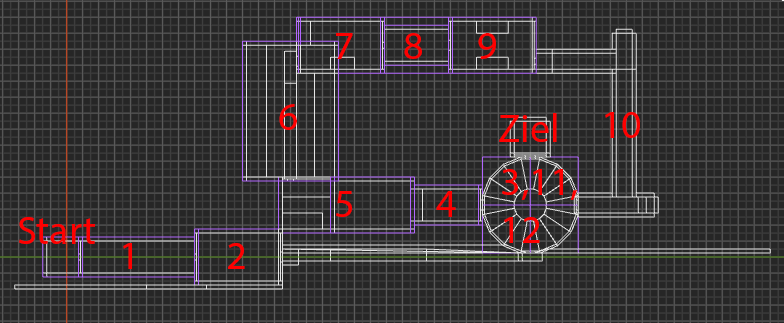
\includegraphics[width=\linewidth]{Assets/Map Layout.png}
    \caption[Grundriss des Kampfabschnitts. Eigene Abbildung.]{Grundriss des Kampfabschnitts mit Raumnummern, Start und Ziel (Draufsicht aus TrenchBroom). Der Kampfabschnitt ist als Rundgang aufgebaut: Raum~12 ist derselbe Raum wie Raum~3, und Raum~11 liegt gleich gross direkt darüber. Deshalb sind die drei Räume an derselben Stelle eingezeichnet. Eigene Abbildung.}
    \label{fig:Map}
\end{figure}

Pro Welle lässt sich zudem festlegen, wie viele Gegner gleichzeitig im Raum sein dürfen (Abschnitt~\ref{sec:V2}). Stirbt ein Gegner, rückt ein weiterer nach. Die Reihenfolge, in der die Gegner erscheinen, ist im Voraus festgelegt. Jede Welle besteht aus einem Teil fest platzierter und einem Teil zufällig erscheinender Gegner (Abschnitt~\ref{sec:V5}). Nachdem alle Wellen eines Raumes besiegt wurden, öffnet sich genau eine Tür, durch die der Spieler weitergehen kann.

Tabelle~\ref{tab:Raeume} zeigt den Aufbau der einzelnen Räume; die Raumtypen werden in Abschnitt~\ref{sec:V6} erläutert.

\begin{table}[H]
    \centering
    \small
    \renewcommand{\arraystretch}{1.3}
    \begin{tabular}{|>{\raggedright\arraybackslash}p{0.9cm}|>{\raggedright\arraybackslash}p{1.6cm}|>{\raggedright\arraybackslash}p{1.1cm}|>{\raggedright\arraybackslash}p{5.5cm}|>{\raggedright\arraybackslash}p{3.6cm}|}
        \hline
        \textbf{Raum} & \textbf{Raumtyp} & \textbf{Wellen} & \textbf{Ablauf} & \textbf{Funktion} \\
        \hline
        1 & Intimate & 2 & Welle 1: ein Soldier. Welle 2: fünf Soldiers, höchstens zwei gleichzeitig. & Einführung des Soldiers; Spiel erklären \\
        \hline
        2 & Intimate & 2 & Welle 1: ein Archer. Welle 2: fünf Archer, höchstens zwei gleichzeitig. & Einführung des Archers \\
        \hline
        3 & Prospect & 3 & Pro Welle insgesamt etwa 10--15 Gegner, gemischt. & Erstmals gemischte Gegnertypen; Formationen und Dilemma (V3) werden vorgestellt \\
        \hline
        4 & Narrow & 3 & Welle 1: ein einzelner Soldier mit Überraschungsangriff. Welle 2: der Heavy Soldier alleine. Welle 3: Heavy Soldier in Kombination mit dem Archer. & Einführung des Heavy Soldiers; erste Plattform (Box), auf der man sich vor den Gegnern ausruhen kann \\
        \hline
        5 & Prospect & 2 & Welle 1: Archer, Soldier, Heavy Soldier. Welle 2: Archer, Soldier. & Üben des Gelernten; neue Hindernisformation \\
        \hline
        6 & Prospect & 3 & \textcolor{red}{[ergänzen]} & Einführung des Heavy Archers; Brücke als neues Hindernis \\
        \hline
        7 & Intimate & 3 & \textcolor{red}{[ergänzen]} & Einführung des Chain Archers \\
        \hline
        8 & Narrow & 3 & \textcolor{red}{[ergänzen]} & \textcolor{red}{[ergänzen]} \\
        \hline
        9 & Intimate & 2 & \textcolor{red}{[ergänzen]} & \textcolor{red}{[ergänzen]} \\
        \hline
        10 & Narrow & 3 & \textcolor{red}{[ergänzen]} & \textcolor{red}{[ergänzen]} \\
        \hline
        11 & Prospect & 1 & \textcolor{red}{[ergänzen]} & \textcolor{red}{[ergänzen]} \\
        \hline
        12 & Prospect & 2 & \textcolor{red}{[ergänzen]} & \textcolor{red}{[ergänzen]} \\
        \hline
    \end{tabular}
    \caption{Aufbau der Räume des Kampfabschnitts}
    \label{tab:Raeume}
\end{table}

\begin{itemize}[leftmargin=1.5cm]
    \item \textcolor{red}{\textbf{Räume 6--12} in der Tabelle ergänzen (Ablauf und Funktion).}
    \item \textcolor{red}{\textbf{Widerspruch:} \enquote{eine Welle kann zwischen 10 und 30 Gegner enthalten} -- in Raum 1, 2 und 4 haben Wellen 1 bzw.\ 5 Gegner. Spannweite anpassen.}
    \item \textcolor{red}{\textbf{Zwölf Räume vs.\ Karte:} Raum~3 und Raum~12 sind derselbe Raum. Klarstellen, ob es zwölf Encounter in elf Räumen sind, und den Rundgang in 1--2 Sätzen beschreiben (Start, \ldots, Drop-in von Raum~11 zurück in die Arena, Ziel). TP2 spricht im Playtest von \enquote{Raum 7.5} -- wie passt das zur Nummerierung?}
    \item \textcolor{red}{\enquote{Stirbt ein Gegner, rückt ein weiterer nach}: Das ist genau das lückenlose Nachrücken aus \game{Ninja Gaiden} (Frage~D1, 3.3.3). Kurzer Rückverweis.}
    \item \textcolor{red}{Das Vorgehen beim Bauen (Greybox, Iterationen) steht schon in Abschnitt~\ref{sec:VorgehenUmsetzung}; hier nur verweisen. Technische Details zum Wellensystem mit Verweis auf die technische Dokumentation.}
    \item \textcolor{red}{Optional: Karte aufwerten (Raumtypen farbig mit Legende, Weg als Pfeile, Drop-in 11$\rightarrow$12, höhere Auflösung). Dann zeigt sie Raumwechsel und Spannungskurve auf einen Blick.}
\end{itemize}

\subsection{Gegnerverhalten und Spieler-Gegner-Interaktion} \label{sec:UmsetzungGegner}

\subsubsection{V1: Überlegenheit als Grundzustand} \label{sec:V1}

\paragraph{Vorschlag und Herleitung}
Der Spieler soll sich seinen Gegnern grundsätzlich überlegen fühlen, wobei dieser Zustand gezielt durchbrochen werden kann. Der Nutzen liegt im Spielgefühl: Aggression soll sich sicher und belohnt anfühlen, während Spannung erst dort entsteht, wo die Kontrolle kurzzeitig bedroht wird. Hergeleitet ist der Vorschlag aus dem Kontrast der beiden Referenzspiele, der dauerhaften Überlegenheit in \game{NieR: Automata} (Abschnitt~\ref{sec:ReferenzspielanalyseNier}) gegenüber dem prekären Gleichgewicht in \game{Ninja Gaiden} (Abschnitt~\ref{sec:ReferenzspielanalyseNinja}), sowie aus dem Prinzip des emotionsgeleiteten Designs (Abschnitt~\ref{sec:Pacing}).

\paragraph{Umsetzung im Prototyp}
Im Eins-gegen-eins ist der Spieler jedem einzelnen Gegner haushoch überlegen. Er hat je nach Gegnertyp etwa 1,5- bis 5-mal so viele Lebenspunkte wie ein einzelner Gegner, mit Ausnahme des Heavy Soldiers, der mit 200 Lebenspunkten genau gleich viele hat. Auch pro Treffer verursacht der Spieler mit 20 bis 40 Schaden meist mehr als die Gegner mit 10 bis 20 Schaden pro Schlag bzw.\ Pfeil; nur der Heavy Soldier liegt mit 30 Schaden im selben Bereich (Tabellen~\ref{tab:Gegnertypen} und~\ref{tab:Combos}). Zudem hat jeder Gegner ein simples Moveset, also nur eine begrenzte Anzahl Bewegungen, die er ausführen kann. Der Spieler hat deutlich mehr: Er kann zum Beispiel schneller rennen, springen, was keiner der Gegner kann, und sich sogar heilen. Ausserdem sind alle Gegner ausser dem Heavy Soldier unterbrechbar, was sie im direkten Nahkampf sehr schwach macht.

Man könnte deshalb annehmen, dass der Spieler auch grosse Mengen von Gegnern problemlos bewältigt. Das stimmt allerdings nicht ganz, denn die Überlegenheit wird an mehreren Stellen gezielt durchbrochen:

\begin{itemize}[leftmargin=1.5cm]
    \item In der Gruppe werden die Gegner von einem zentralen Gegnermanager koordiniert und stellen so eine grössere Gefahr dar (Abschnitte~\ref{sec:V2} und~\ref{sec:V3}).
    \item Einige Gegner lassen sich nicht mit einer einzigen Combo besiegen, was grosse Horden zusätzlich gefährlich macht.
    \item Am Ende einer Combo weist der Spieler eine gewisse Trägheit auf. Wird der Gegner mit der Combo nicht besiegt, erhält dieser dadurch die Möglichkeit, den Spieler zu treffen.
    \item Das Heilen dauert eine gewisse Zeit. Gibt es zu wenig Platz und keine Möglichkeit, sich zu verstecken, ist es sehr schwer, sich zu heilen (vgl. Abschnitt~\ref{sec:V6}).
\end{itemize}

Als Alternative haben wir versucht, die Encounters durch mehr Lebenspunkte der Gegner sowie durch mehr und längere Wellen schwieriger zu machen. Wir haben uns aber gegen diese Lösungen entschieden, da sie das Spiel nur sinnlos strecken und keinen Mehrwert bieten. Zudem verlangsamen sie den Spielfluss, der nach unserer Vorstellung schnell und aggressiv sein soll (Abschnitt~\ref{sec:Genredefinition}).

\begin{itemize}[leftmargin=1.5cm]
    \item \textcolor{red}{\enquote{haushoch überlegen} ist umgangssprachlich, besser \enquote{deutlich überlegen}.}
    \item \textcolor{red}{\textbf{Rückbezug:} Dass sich der Heavy Soldier nicht unterbrechen lässt, ist genau die Idee aus \game{Ninja Gaiden} (3.3.3). Einen Halbsatz bei \enquote{alle Gegner ausser dem Heavy Soldier unterbrechbar} ergänzen.}
    \item \textcolor{red}{\textbf{Springen:} Hier und in V3 steht, dass kein Gegner springen kann. TP5 sagt im Playtest, der Heavy Soldier \enquote{springe einfach irgendwohin} (Anhang, TP5 B11). Prüfen, ob eine Angriffsanimation so wirkt, und präzisieren.}
    \item \textcolor{red}{Optional: Wie füllt sich die Manaleiste wieder auf? TP5 starb, weil das Mana fehlte; ohne diese Information versteht man das in Kapitel~\ref{sec:Evaluation} nicht.}
\end{itemize}

\paragraph{Überprüfbarkeit}
\begin{itemize}[leftmargin=1.5cm]
    \item \textcolor{red}{\textbf{Überprüfbarkeit:} Szene, Datei oder Klasse nennen bzw.\ auf das passende Kapitel der technischen Dokumentation verweisen.}
\end{itemize}

\subsubsection{V2: Begrenzung gleichzeitiger Angreifer} \label{sec:V2}

\paragraph{Vorschlag und Herleitung}
Auch bei vielen Gegnern sollen nie alle gleichzeitig angreifen, sondern nur eine begrenzte Zahl. Der Nutzen betrifft Schwierigkeit und Spielfluss, da grosse Gruppen dadurch lesbar und fair bleiben, statt den Spieler zu überfordern. Beide Referenzspiele nutzen dieses Mittel, in \game{Ninja Gaiden} mit maximal etwa vier aktiven Gegnern, in \game{NieR: Automata} mit vermutlich höchstens zwei gleichzeitig angreifenden Nahkämpfern (Abschnitt~\ref{sec:Vergleich}), und es entspricht dem Pacing-Gedanken der Recherche (Abschnitt~\ref{sec:Pacing}).

\paragraph{Umsetzung im Prototyp}
Im Prototyp wird die Zahl gleichzeitig angreifender Gegner auf zwei Ebenen reguliert. Erstens lässt sich für jede Welle festlegen, wie viele ihrer Gegner gleichzeitig im Raum sein dürfen (zum Wellensystem siehe Abschnitt~\ref{sec:Kampfabschnitt}). Hat eine Welle beispielsweise 30 Gegner und sind höchstens sechs gleichzeitig erlaubt, befinden sich nur sechs im Raum; erst wenn einer stirbt, rückt ein weiterer nach. Zweitens lässt sich, vereinfacht gesagt, einstellen, wie aggressiv eine Welle ist, also wie viele der Gegner sich im Angriffsmodus und wie viele im Abstandsmodus befinden.

Gesteuert wird dies von einem zentralen Gegnermanager, der jederzeit weiss, wie viele Gegner gerade angreifen oder Abstand halten. Über einen Wert lässt sich einstellen, wie viele Gegner angreifen sollen; genau so viele greifen dann auch an.

Typischerweise sind in unserem Spiel drei bis sechs Gegner gleichzeitig am Leben, in Ausnahmefällen auch nur einer oder bis zu acht. Von diesen greifen meistens alle gleichzeitig an, da wir den Gegnermanager sehr aggressiv eingestellt haben.

Gegner, die nicht angreifen, halten einen gewissen Abstand zum Spieler und umkreisen ihn, falls möglich. Archers, die sich nicht bewegen können, bleiben stehen.

Die Grenzwerte sowie die Anzahl der Gegner und Wellen haben wir je nach Raumgrösse festgelegt und so lange angepasst, bis sie uns überzeugt haben.

\begin{itemize}[leftmargin=1.5cm]
    \item \textcolor{red}{\textbf{Zentraler Widerspruch:} Der Vorschlag verlangt, dass \enquote{nie alle gleichzeitig angreifen}, umgesetzt greifen aber meistens alle an. Die eigentliche Begrenzung läuft bei euch über die Zahl gleichzeitig lebender Gegner (3--6, max.\ 8), was ungefähr den etwa vier aktiven Gegnern in \game{Ninja Gaiden} entspricht. Entweder den Vorschlag so formulieren (\enquote{begrenzte Zahl gleichzeitig aktiver Gegner}) oder die Abweichung als bewusste Entscheidung begründen und in Kapitel~\ref{sec:Evaluation} diskutieren. Die Begründung in V4 hängt daran.}
    \item \textcolor{red}{\textbf{Rückbezug auf \game{Ninja Gaiden} (M2):} Angriffs- und Abstandsmodus sind eine vereinfachte Form des Rollensystems aus der Analyse (angreifende Gegner $\approx$ Nahkämpfer, umkreisende $\approx$ Flankierer). Ein Satz dazu beantwortet auch die offene Frage bei V3.}
    \item \textcolor{red}{Herleitung: \enquote{entspricht dem Pacing-Gedanken der Recherche} streichen (siehe Notiz zur Tabelle).}
    \item \textcolor{red}{\enquote{bis sie uns überzeugt haben}: Kriterien nennen -- worauf habt ihr beim Testen geachtet?}
    \item \textcolor{red}{Gilt die Begrenzung auch für die Archers bzw.\ ihre Projektile?}
\end{itemize}

\paragraph{Überprüfbarkeit}
\begin{itemize}[leftmargin=1.5cm]
    \item \textcolor{red}{\textbf{Überprüfbarkeit:} Szene, Datei oder Klasse nennen bzw.\ auf das passende Kapitel der technischen Dokumentation verweisen.}
\end{itemize}

\subsubsection{V3: Ein taktisches Dilemma durch zwei Gegnerrollen} \label{sec:V3}

\paragraph{Vorschlag und Herleitung}
Der Kampfabschnitt soll Nah- und Fernkämpfer kombinieren, sodass der Spieler entscheiden muss, welche Bedrohung er zuerst ausschaltet. Der Nutzen liegt in der Schwierigkeit, die dadurch taktisch statt rein mechanisch (etwa durch mehr Lebenspunkte der Gegner) entsteht und schon kleine Gruppen anspruchsvoll macht. Grundlage ist, dass genau diese Kombination in beiden Referenzspielen den taktischen Druck trägt (Frage~D2 beider Analysen), sowie das Prinzip der Gegnerrollen im Encounter-Design (Abschnitt~\ref{sec:Encounter}).

\paragraph{Umsetzung im Prototyp}
Wie in Abschnitt~\ref{sec:Gegnertypen} beschrieben, gibt es im Prototyp zwei Nah- und drei Fernkämpfer. Den Nahkämpfern kann man, wenn man will, einfach davonrennen, da sie den Spieler nur verfolgen, nicht springen können und langsamer sind als er. Bei den Fernkämpfern geht das nicht, weil sie den Spieler nicht verfolgen, sondern beschiessen. Deshalb stellen die Archers eine grosse Gefahr dar.

Dass der Spieler die Archers nicht einfach einen nach dem anderen besiegen kann, liegt daran, dass sich meistens ein Nahkämpfer zwischen Spieler und Archer befindet, weil sich die Nahkämpfer bewegen und so dazwischenkommen. Deshalb ist der Spieler oft gezwungen, zuerst die Nahkämpfer auszuschalten. Das gibt den Archers allerdings Zeit, auf den Spieler zu schiessen, was wiederum ein weiterer Grund ist, weshalb der Spieler die Archers zuerst besiegen möchte.

Verstärkt wird dieses Dilemma durch die Platzierung der Archers, die oft hinter den Soldiers und weit weg vom Spieler erscheinen, sodass der Spieler sie nicht sofort besiegen kann (Abschnitt~\ref{sec:V5}).

\begin{itemize}[leftmargin=1.5cm]
    \item \textcolor{red}{\textbf{Überschrift und Herleitung:} \enquote{zwei Gegnerrollen} $\rightarrow$ Nah- und Fernkämpfer (siehe Notiz zur Tabelle). \enquote{Prinzip der Gegnerrollen im Encounter-Design (Abschnitt~\ref{sec:Encounter})} ersetzen durch den Verweis auf \game{NieR} D2.}
    \item \textcolor{red}{\textbf{Rückbezug:} Dass Soldiers zwischen Spieler und Archers geraten, ist dieselbe Situation wie mit den Small Stubbies in \game{NieR} (Frage~D2, 3.3.3). Kurz nennen.}
    \item \textcolor{red}{Rollensystem: Wenn ihr es bei V2 als vereinfachte Form beschreibt, reicht hier ein Verweis auf Abschnitt~\ref{sec:V2}.}
\end{itemize}

\paragraph{Überprüfbarkeit}
\begin{itemize}[leftmargin=1.5cm]
    \item \textcolor{red}{\textbf{Überprüfbarkeit:} Szene, Datei oder Klasse nennen bzw.\ auf das passende Kapitel der technischen Dokumentation verweisen.}
\end{itemize}

\subsubsection{V4: Klar telegrafierte Angriffe} \label{sec:V4}

\paragraph{Vorschlag und Herleitung}
Bevorstehende Gegnerangriffe sollen deutlich angekündigt werden, etwa durch sichtbare Vorzeichen. Der Nutzen betrifft Schwierigkeit und Spielgefühl, weil der Spieler auch im Gruppenkampf rechtzeitig reagieren kann und Treffer als eigene Fehler statt als Willkür erlebt. Vorbild ist das deutliche Telegrafieren in \game{NieR: Automata} (Frage~M2), theoretisch gestützt durch das Prinzip der Lesbarkeit (Abschnitt~\ref{sec:Encounter}).

\paragraph{Umsetzung im Prototyp}
Alle unsere Gegner kündigen ihre Angriffe visuell an. Dies geschieht allerdings ausschliesslich über die Animation, nicht über Soundeffekte oder Partikeleffekte: Bevor ein Gegner zuschlägt, wird immer eine kurze Animation abgespielt. Zudem lassen sich die Angriffe, zum Beispiel jene des Soldiers, durch sein Verhalten vorhersagen: Sobald er beim Spieler ankommt, hält er kurz inne und schlägt dann zu. Dieses sehr einfache Muster kann der Spieler beobachten.

Auch der Archer spielt vor dem Schuss eine Ausholanimation ab (\enquote{Anlauf nehmen}). Wie lange es zwischen dem Beginn der Animation und dem Treffer dauert, ist je nach Gegnertyp unterschiedlich: Für jeden Typ haben wir einen Richtwert festgelegt und zusätzlich eine zufällige Zeit dazugerechnet.

Wir haben uns dagegen entschieden, neben den Animationen weitere audiovisuelle Anzeichen umzusetzen, weil uns zum einen die Zeit gefehlt hat und zum anderen so viele Gegner gleichzeitig angreifen, dass es keine grosse Rolle spielt, ob ein einzelner Gegner angreift. Entscheidend ist die Menge der Gegner, nicht der einzelne Gegner.

\begin{itemize}[leftmargin=1.5cm]
    \item \textcolor{red}{\textbf{Argument prüfen:} \enquote{so viele Gegner greifen gleichzeitig an, dass es keine grosse Rolle spielt} widerspricht V2 und dem Ziel von V4 selbst. Ehrlicher: bewusste Priorisierung aus Zeitgründen. In Kapitel~\ref{sec:Evaluation} mit Q4 und B4 diskutieren (TP4 vermisste Sound-Hinweise).}
    \item \textcolor{red}{Herleitung: \enquote{theoretisch gestützt durch das Prinzip der Lesbarkeit} streichen oder abschwächen (siehe Notiz zur Tabelle). \game{NieR} M2 reicht, und es steht jetzt auch in 3.3.3.}
    \item \textcolor{red}{Gilt die Ausholanimation für alle drei Fernkämpfer? Richtwerte und Grösse des Zufallsanteils nennen (z.\,B.\ in Sekunden).}
    \item \textcolor{red}{Optional: Screenshot einer Ankündigungsanimation (\enquote{Eigene Abbildung}).}
\end{itemize}

\paragraph{Überprüfbarkeit}
\begin{itemize}[leftmargin=1.5cm]
    \item \textcolor{red}{\textbf{Überprüfbarkeit:} Szene, Datei oder Klasse nennen bzw.\ auf das passende Kapitel der technischen Dokumentation verweisen.}
\end{itemize}

\subsection{Levelaufbau und Gegnerplatzierung} \label{sec:UmsetzungLevel}

\subsubsection{V5: Lesbare Platzierung, dynamisches Verhalten} \label{sec:V5}

\paragraph{Vorschlag und Herleitung}
Gegner sollen zu Beginn lesbar und teils symmetrisch platziert sein, sich danach aber dynamisch verhalten, etwa den Spieler umzingeln. Der Nutzen betrifft Spielfluss und Spielgefühl: Die Anfangsaufstellung gibt Überblick, das anschliessende Verhalten hält den Kampf unter Druck und unvorhersehbar. Der Vorschlag verbindet die durchdachte, manuelle Platzierung aus \game{NieR: Automata} (Frage~A3) mit dem dynamischen Verhalten aus \game{Ninja Gaiden} (Frage~D3, Abschnitt~\ref{sec:Vergleich}) und stützt sich auf die Prinzipien der Lesbarkeit und der Gegner als raumbildende Elemente (Abschnitt~\ref{sec:Encounter}).

\paragraph{Umsetzung im Prototyp}
Besonders die erste Aufstellung der Gegner zu Beginn einer Welle haben wir oft manuell festgelegt, um eine Symmetrie in die Platzierung zu bringen. Die meisten Soldiers erscheinen dagegen zufällig, da sie sich bewegen können und ihre Startposition während des Kampfgeschehens deshalb keine allzu grosse Rolle spielt. Die Archers platzieren wir manuell, eher an den Rändern der Räume oder auf Hindernissen (Abschnitt~\ref{sec:V6}). Dadurch befinden sich oft Soldiers zwischen dem Spieler und den Archers, was das Dilemma aus Abschnitt~\ref{sec:V3} verstärkt.

Von ausserhalb des Raumes ist die erste Aufstellung allerdings nicht sichtbar, da die Gegner erst erscheinen, nachdem der Spieler den Raum betreten hat. Einen Eindruck der Raumgeometrie kann sich der Spieler jedoch schon vorher verschaffen.

Nach der Anfangsaufstellung verhalten sich die Gegner dynamisch: Gegner, die gerade nicht angreifen, halten Abstand zum Spieler und umkreisen ihn (Abschnitt~\ref{sec:V2}).

\begin{itemize}[leftmargin=1.5cm]
    \item \textcolor{red}{\textbf{Herleitung:} \enquote{Gegner als raumbildende Elemente} $\rightarrow$ \textit{Shrinking Fortress}, wie in 4.2 und 4.7.}
    \item \textcolor{red}{\textbf{Klären:} Bezieht sich \enquote{die meisten Soldiers erscheinen zufällig} auf die nachrückenden Gegner oder auch auf die erste Aufstellung? Sonst widerspricht es dem ersten Satz.}
    \item \textcolor{red}{\textbf{Ehrlich ergänzen:} TP3 bemerkte im Playtest, dass Gegner ausserhalb des Sichtfelds erscheinen (Abschnitt~\ref{sec:ErgVorschlag}). Wenn zufällige Soldiers auch hinter dem Spieler erscheinen können, das hier so schreiben -- das ist das Prinzip aus \game{Ninja Gaiden} (Frage~A3).}
    \item \textcolor{red}{\textbf{Lesbarkeit:} Die Gegner erscheinen erst nach dem Betreten des Raumes. Das widerspricht dem Prinzip \enquote{Kampfraum vom Eingang aus lesbar} (4.2). Kurz begründen (z.\,B.\ technisch einfacher, Überraschung) und in 6.4 aufgreifen.}
    \item \textcolor{red}{Optional: Abbildung mit eingezeichneten Spawnpunkten (z.\,B.\ Raum~3).}
\end{itemize}

\paragraph{Überprüfbarkeit}
\begin{itemize}[leftmargin=1.5cm]
    \item \textcolor{red}{\textbf{Überprüfbarkeit:} Szene, Datei oder Klasse nennen bzw.\ auf das passende Kapitel der technischen Dokumentation verweisen.}
\end{itemize}

\subsubsection{V6: Der Raum als Druckmittel} \label{sec:V6}

\paragraph{Vorschlag und Herleitung}
Die Grösse des Kampfraums soll gezielt zwischen Enge und Weite wechseln. Der Nutzen liegt in der Schwierigkeit, da ein enger Raum den Spieler zu methodischerem Spiel zwingt, während ein weiter Raum ihm taktische Distanz erlaubt. Vorbild ist die gezielte Raumverengung in \game{Ninja Gaiden} (Frage~M3), theoretisch untermauert durch die räumlichen Typologien Narrow und Prospect Space (Abschnitt~\ref{sec:Raumtypologien}).

\paragraph{Umsetzung im Prototyp}
In unserem Spiel gibt es eine Mischung aus den drei Raumtypen Narrow, Intimate und Prospect Space (Abschnitt~\ref{sec:Raumtypologien}). Jeder dieser Typen hat für den Spieler Vor- und Nachteile; Tabelle~\ref{tab:Raeume} zeigt die Zuordnung aller Räume.

\textbf{Intimate Spaces} sind Räume, in denen der Spieler genug Platz hat, sich zu bewegen und sein komplettes Moveset auszunutzen. In diesen Räumen ist der Spieler am stärksten im Vorteil. Nur vier unserer Räume fallen in diese Kategorie, nämlich die Räume 1, 2, 7 und 9. Die Räume 1 und 2 sind Intimate Spaces, weil hier die Kampfmechaniken beigebracht und die ersten Gegner vorgestellt werden; die Räume 7 und 9 sind es aufgrund der Spannungskurve.

\textbf{Narrow Spaces} sind, wie der Name sagt, enge Räume, in denen sich das Moveset des Spielers nicht vollständig entfalten kann. Davon haben wir drei, nämlich die Räume 4, 8 und 10. In Narrow Spaces sind eher die Nahkämpfer im Vorteil. Da unser Spiel besonders auf aggressive und schnelle Action ausgelegt ist, ergibt es wenig Sinn, viele enge Räume einzubauen, in denen man eher genau, taktisch und zurückhaltend spielen muss. Dennoch tragen sie zur Spannungskurve bei, weshalb wir einige davon haben.

\textbf{Prospect Spaces} sind die restlichen Räume 3, 5, 6, 11 und 12. Sie zeichnen sich dadurch aus, dass sie riesig sind und mehr als genug Platz bieten, um das Moveset des Spielers zu unterstützen. Sie sind sogar so gross, dass sie den Spieler verwundbar machen: Hier ist er den Archers eher unterlegen, da diese aus der Ferne angreifen können.

Die Räume einer Kategorie sind allerdings nicht zwangsläufig gleich gross. Ausschlaggebend für die Einordnung ist, wie gut sich der Spieler in einem Raum bewegen kann, und das hängt neben der Grösse von weiteren Variablen ab, vor allem von der Anzahl und den Typen der Gegner. So kann ein Raum riesig, aber dennoch ein Intimate und kein Prospect Space sein, weil in ihm nur wenige Gegner gleichzeitig erscheinen oder eher wenige Archers vorkommen.

In den Räumen befinden sich zudem Hindernisse, vor allem Boxen bzw.\ Container und in Raum~6 eine Brücke. Auf diesen erscheinen meistens die Archers, was es dem Spieler erschwert, an sie heranzukommen, und den Archers einen guten Überblick verschafft. Gleichzeitig können die Hindernisse dem Spieler als Deckung dienen. Der Spieler kann auch auf eine Box steigen, um sich zu heilen, da die Soldiers nicht springen können.

\begin{itemize}[leftmargin=1.5cm]
    \item \textcolor{red}{\textbf{Eigene Anpassung von Totten kennzeichnen:} Bei Totten werden die Raumtypen über Raumwirkung und Grösse definiert, bei euch über die Bewegungsfreiheit inklusive Anzahl und Art der Gegner. Das ist legitim und jetzt durch 4.7 gestützt (Shrinking Fortress; Rogers: Gegnerzahl passend zur Raumgrösse). Einen Satz mit Verweis auf Abschnitt~\ref{sec:ZwischenfazitLD} ergänzen.}
    \item \textcolor{red}{\textbf{Hindernisse:} Boxen und Brücke mit 4.2 verbinden (Höhenunterschiede, Deckung, Flankiermöglichkeiten; Horizon-Talk).}
    \item \textcolor{red}{\enquote{aufgrund der Spannungskurve} (Räume 7 und 9) kurz erklären, z.\,B.\ als Entlastung nach einem Narrow Space (Raum~8)?}
    \item \textcolor{red}{Auf die Karte (Abbildung~\ref{fig:Map}) verweisen.}
    \item \textcolor{red}{\textbf{Für Kapitel~\ref{sec:Evaluation} vormerken:} Raum~11 ist gross und hat nur eine Welle; TP3 erwartete dort einen Boss. Das passt zu Totten, laut dem Prospect Spaces oft Bossräume sind (4.3).}
\end{itemize}

\paragraph{Überprüfbarkeit}
\begin{itemize}[leftmargin=1.5cm]
    \item \textcolor{red}{\textbf{Überprüfbarkeit:} Szene, Datei oder Klasse nennen bzw.\ auf das passende Kapitel der technischen Dokumentation verweisen.}
\end{itemize}

\subsubsection{V7: Wellenstruktur mit Erholungsphasen} \label{sec:V7}

\paragraph{Vorschlag und Herleitung}
Der Kampfabschnitt soll in Wellen mit kontrollierter Eskalation und kurzen Erholungsphasen dazwischen aufgebaut sein. Der Nutzen betrifft den Spielfluss, indem sich Anspannung und Entlastung abwechseln und die Schwierigkeit planbar ansteigt. Beide Referenzspiele nutzen dieses Muster (Frage~D1 in \game{Ninja Gaiden}, Frage~A4 in \game{NieR: Automata}), das der Recherche als Rollercoaster-Pacing bekannt ist (Abschnitt~\ref{sec:Pacing}).

\paragraph{Umsetzung im Prototyp}
Wie die Wellen technisch funktionieren, ist in Abschnitt~\ref{sec:Kampfabschnitt} beschrieben. Unser Prototyp weist eine zweifache Wellenstruktur auf: zum einen von Raum zu Raum und zum anderen, offensichtlicher, von Welle zu Welle. Die Spannungskurve entwickelt sich entsprechend auf beiden Ebenen: In den meisten Räumen gibt es einfachere und schwerere Wellen, und es gibt Räume, die insgesamt schwerer oder einfacher sind.

Die Schwierigkeit steigt mit der Anzahl der Gegner und mit der Einführung neuer Gegnertypen (Abschnitt~\ref{sec:V8}). Besonders deren Kombination im Raum erhöht die Schwierigkeit.

Am Ende eines Raumes kann sich der Spieler immer so lange erholen, wie er möchte, bevor er in den nächsten Raum geht. Zwischen den Wellen gibt es dagegen nicht viel Erholungszeit, denn die nächste Welle erscheint direkt, nachdem alle Gegner der vorherigen besiegt wurden. Abgesehen von leichteren Wellen besteht die einzige Erholungsmöglichkeit hier darin, den letzten Gegner am Leben zu lassen und sich so selbst Erholungszeit zu verschaffen. Innerhalb eines Raumes kann man sich zudem auf den Boxen ausruhen, sofern man diese von Gegnern befreit hat (Abschnitt~\ref{sec:V6}).

\begin{itemize}[leftmargin=1.5cm]
    \item \textcolor{red}{\textbf{Rückbezug:} Die zweifache Wellenstruktur (Raum zu Raum, Welle zu Welle) ist genau das fraktalähnliche Rollercoaster-Pacing aus 4.4 und 4.7. Einen Halbsatz mit Verweis ergänzen.}
    \item \textcolor{red}{\textbf{Widerspruch:} Der Vorschlag verlangt \enquote{kurze Erholungsphasen} zwischen den Wellen, umgesetzt gibt es kaum welche. Bewusst so? Kurz begründen und in Kapitel~\ref{sec:Evaluation} diskutieren (TP2 fand es schwer, Heilpausen zu finden).}
    \item \textcolor{red}{\enquote{Den letzten Gegner leben lassen}: beabsichtigt oder von euch bzw.\ den Testpersonen entdeckt? Klarstellen.}
    \item \textcolor{red}{Optional: Diagramm der geplanten Spannungskurve über die Räume 1--12.}
\end{itemize}

\paragraph{Überprüfbarkeit}
\begin{itemize}[leftmargin=1.5cm]
    \item \textcolor{red}{\textbf{Überprüfbarkeit:} Szene, Datei oder Klasse nennen bzw.\ auf das passende Kapitel der technischen Dokumentation verweisen.}
\end{itemize}

\subsubsection{V8: Gestaffelte Einführung neuer Gegner} \label{sec:V8}

\paragraph{Vorschlag und Herleitung}
Jeder neue Gegnertyp soll zuerst isoliert auftreten und erst danach mit anderen kombiniert werden. Der Nutzen betrifft Spielfluss und Schwierigkeit, weil der Spieler einen Gegner in Ruhe verstehen kann, bevor die Kombination ihn fordert. Grundlage ist das Scaffolding-Prinzip (Abschnitt~\ref{sec:Scaffolding}) sowie die entsprechende Struktur in \game{NieR: Automata} (Frage~D1).

\paragraph{Umsetzung im Prototyp}
Wie Tabelle~\ref{tab:Raeume} zeigt, werden unsere fünf Gegnertypen in den Räumen 1, 2, 4, 6 und 7 vorgestellt. In den Räumen 1 und 2 wollen wir die Basisgegner vorstellen und gleichzeitig das Spiel erklären. Sobald sich der Spieler an das Neue gewöhnt hat, folgt ein neuer Gegnertyp. Gleichzeitig wollten wir alle Gegner früh genug vorgestellt haben, um anschliessend verschiedene Kombinationen mit ihnen ausprobieren zu können.

Der Heavy Soldier wurde im ersten Narrow Space (Raum~4) eingeführt, um ihn noch bedrohlicher wirken zu lassen. Der Heavy Archer wurde hingegen in einem Prospect Space (Raum~6) vorgestellt, da er sich besonders in grossen Räumen als bedrohlich erweist. Der Chain Archer wurde in einem Intimate Space (Raum~7) vorgestellt, um dem Soldier im Raumtyp, in dem der Spieler die grössten Vorteile hat, etwas den Platz streitig zu machen.

Damit halten wir uns an unsere Recherche, nach der pro Raum etwa eine neue Mechanik eingeführt werden sollte, um den Spieler nicht zu stark zu belasten und das Spiel dennoch unterhaltsam zu gestalten (Abschnitt~\ref{sec:Scaffolding}).

\begin{itemize}[leftmargin=1.5cm]
    \item \textcolor{red}{\textbf{Muss angepasst werden:} \enquote{Damit halten wir uns an unsere Recherche, nach der pro Raum etwa eine neue Mechanik eingeführt werden sollte, um den Spieler nicht zu stark zu belasten und das Spiel dennoch unterhaltsam zu gestalten.} Die Quelle sagt \enquote{pro Level}, und die Begründung (Belastung, Unterhaltung) steht nicht in 4.5. Wie in 4.7 formulieren: Grundsatz \enquote{pro Level}, von euch auf einzelne Räume übertragen; die Begründung als eure eigene kennzeichnen.}
    \item \textcolor{red}{\enquote{um dem Soldier etwas den Platz streitig zu machen}: gemeint ist wohl \emph{dem Spieler}? Prüfen.}
    \item \textcolor{red}{\textbf{Braiding} (4.5): kurz nennen, wo die neuen Typen erstmals mit anderen kombiniert werden (z.\,B.\ Raum~3; Raum~4: Heavy Soldier + Archer).}
    \item \textcolor{red}{Zeitform: \enquote{wollen wir vorstellen} und \enquote{wollten} im selben Absatz -- einheitlich in der Vergangenheit.}
\end{itemize}

\paragraph{Überprüfbarkeit}
\begin{itemize}[leftmargin=1.5cm]
    \item \textcolor{red}{\textbf{Überprüfbarkeit:} Szene, Datei oder Klasse nennen bzw.\ auf das passende Kapitel der technischen Dokumentation verweisen.}
\end{itemize}

\end{document}
